\documentclass[tikz,border=6pt]{standalone}
\usepackage{amsmath,amssymb}
\usepackage{xcolor}
\definecolor{accent}{HTML}{A13D2C}
\definecolor{accent2}{HTML}{2B5F6B}
\definecolor{muted}{HTML}{5A564F}
\definecolor{panel}{HTML}{F8F6F0}
\definecolor{linecol}{HTML}{D8D2C4}
\definecolor{astroblue}{HTML}{1B4F72}
\usetikzlibrary{calc,arrows.meta}
\begin{document}
% Exact pressure-free collapse of a uniform sphere: R = R0 cos^2(xi), t/t_ff = (xi + sin xi cos xi)/(pi/2).
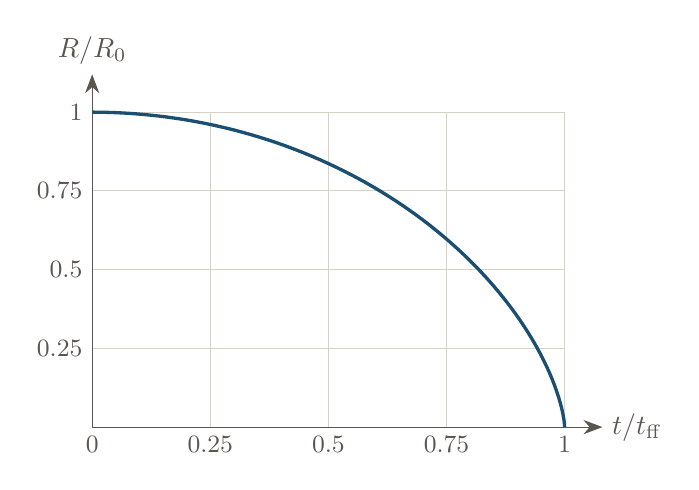
\begin{tikzpicture}[x=6cm,y=4cm, >={Stealth[length=2.4mm]}]
  \draw[linecol] (0,0) grid[xstep=0.25,ystep=0.25] (1,1);
  \draw[->, muted] (0,0) -- (1.08,0) node[right] {$t/t_{\rm ff}$};
  \draw[->, muted] (0,0) -- (0,1.12) node[above] {$R/R_0$};
  \foreach \x in {0,0.25,0.5,0.75,1} \node[below, muted] at (\x,0) {\small \x};
  \foreach \y in {0.25,0.5,0.75,1} \node[left, muted] at (0,\y) {\small \y};
  \draw[astroblue, line width=1.2pt, domain=0:90, samples=200, variable=\t]
    plot ({(rad(\t)+sin(\t)*cos(\t))/(pi/2)}, {cos(\t)^2});
\end{tikzpicture}
\end{document}
